
Em primeira instância, foram geradas matrizes $A$ e $B$ de maneira aleatória apartir da distribuição gaussiana, o que ocasionou em um resultado semelhante de aproximação para a amostragem utilizando as probabilidades encontradas na seção anterior desse documento e utilizando uma distribuição uniforme visto que, sendo as matrizes $A$ e $B$ geradas a partir de uma gaussiana centrada no zero, a norma de todas as colunas de $A$ é bem semelhante, e o mesmo se aplica para todas as linhas de $B$, resultando em uma distribuição de probabilidade naturalmente semelhante à uniforme.

\begin{figure}[H]
  \centering
  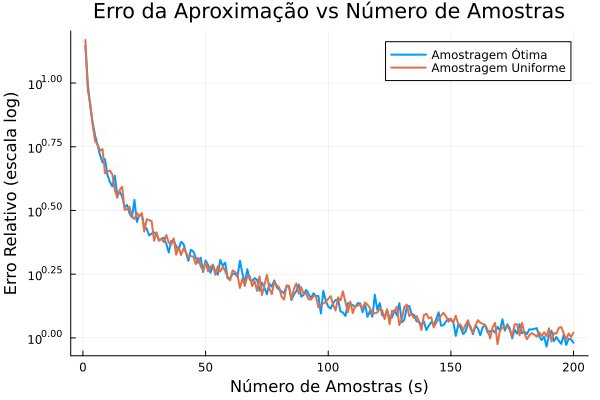
\includegraphics[width=0.8\textwidth]{first-experiment.png}
  \caption{Erro relativo da aproximação do produto $AB$ via amostragem probabilística.}
  \label{fig:first-experiment}
\end{figure}

Em seguida, realizamos os testes gerando as matrizes $A$ e $B$ a partir de matrizes com distribuição uniforme e escalando os resultados obtidos por pesos entre $0.1$ e $100$, ocasionando em matrizes com colunas com normas com maior variação, resultando assim em um experimento que apresenta o resultado esperado.

\begin{figure}[H]
  \centering
  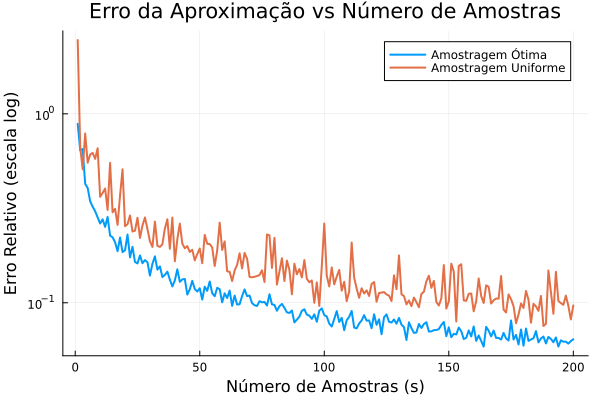
\includegraphics[width=0.8\textwidth]{second-experiment.png}
  \caption{Erro relativo da aproximação do produto $AB$ via amostragem probabilística.}
  \label{fig:second-experiment}
\end{figure}

Ambas as imagens representam no eixo $y$ o erro relativo de aproximação obtido (em escala logarítmica), calculado pela fórmula \[\dfrac{\fnorm{AB - \bar{AB}}}{\fnorm{AB}},\] e no eixo $x$ o número de mostras. Outro ponto importante de se notar é que o erro apresenta a tendência de diminuir conforme o número de amostras aumenta.
